\chapter{Backgrounds}
\label{chap:backgrounds}
	\textit{introduces the background knowledge of this thesis, including the information about API, Web Application Firewall, Machine Learning Model and Deep Neural Network}
\minitoc

\section{Web Application Firewall} 
\label{sec:waf}
	
\subsection{What is WAF ?}
\label{subsec:waf_def}
WAF stands for \textbf{Web Application Firewall}. This firewall solution commonly monitors data packets and filters them for the presence of malware or viruses. It performs the data monitoring/filtering for to and from data packets.  

The WAF tool can be distributed using network-based, cloud-based, or host-based architectures. It needs a reverse proxy to make sure that one or more web apps are in front of it while facing forward. 

It can be utilized either alone or in conjunction with other applications. WAF may function at a lower level or a higher level depending on the requirement\footnote{Wallarm. \textit{WAF Meaning}. \url{https://www.wallarm.com/what/waf-meaning}}.


\subsection{How does WAF work?}
\label{subsec:waf_work}
As mentioned before, WAF is placed at the application layer and functions as a two-way protection there. At work, WAF keeps an eye on HTTP or HTTPS traffic entering or leaving a certain web app. When a malicious object is seen in the traffic, WAF activates and destroys it. \\
\begin{figure}[!h]
   
	\centering
	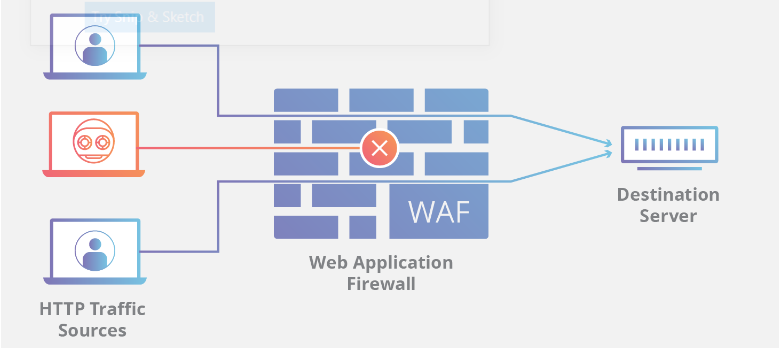
\includegraphics[width=\linewidth, height=10cm,keepaspectratio]{figures/WAF.JPG}
	\caption{Normal users (top-left and bottom-left) are permitted access to the server with a WAF enabled, but attackers (middle-left) are prevented from doing so.}\label{Fig:Data1}
  
\end{figure}
\\
To make the process a bit more simplified, WAF predefined what is vindictive and what’s not. WAF follows these rules all through the process. Mainly, WAF analyses the GET and POST part of the HTTP traffic. GET retrieves data from the server while POST is used to guide the data to the server to alter its original condition\footnote{Wallarm. \textit{WAF Meaning}. \url{https://www.wallarm.com/what/waf-meaning}}.

\subsection{WAF vs Firewall}
\label{subsec:versus}
The firewall and WAF appear to be similar on the surface. They also share a
number of characteristics with one another. However, they are not the same. There are some key distinctions. Understanding the differences is crucial if you’re going to put anyone into action. A firewall is a general phrase that refers to a variety of firewalls used to safeguard computer networks. It filters the data packets while it is in use. Based on the security they provide and their delivery method, firewalls can be differentiated from one another. For example, only a small number of firewalls employ packet filtering, whereas others make use of proxies, NGFW, or stateful inspection. In comparison to proxy firewalls, WAF. However, there is a distinction. The system is not protected from assaults that occur on a fundamental level by a firewall. The WAF concentrates on Layer 7 logic.

Web application firewalls, or WAFs, are primarily used to protect web applications from online threats. Work on it starts at the application layer. Therefore, WAF implementation is always done at the application layer, regardless of the strategy\footnote{Wallarm. \textit{WAF Meaning}. \url{https://www.wallarm.com/what/waf-meaning}}. 
	\begin{figure}[h!]
		\centering
		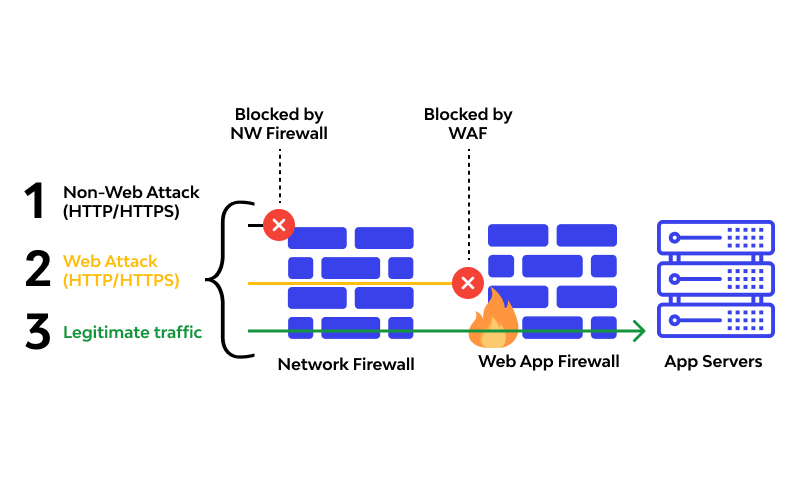
\includegraphics[width=\linewidth, height=10cm,keepaspectratio]{figures/waf3.png}
		\caption{Comparison between WAF and network firewall}
	\end{figure}

% \subsection{Receptive field} 
% \label{subsec:receptive_field}
% 	Receptive field\index{Receptive field} trong lĩnh vực thị giác máy tính được định nghĩa là vùng trên không gian đầu vào tương ứng cho một đặc trưng được trích xuất ở kết quả đầu ra. Receptive field của một đặc trưng được mô tả bằng điểm chính giữa và kích thước của nó.  Trong một receptive field, điểm ảnh càng gần tâm càng đóng góp nhiều vào đặc trưng đầu ra. Điều đó có nghĩa rằng, một đặc trưng không chỉ nhìn vào một vùng riêng biệt trong ảnh đầu vào mà còn tập trung nhiều vào vùng giữa của receptive field đó. 
	
% 	\autoref{fig:receptive_field} minh họa receptive field của toán tử convolution có kích thước filter\index{Filter} $3\times3$, stride\index{Stride} là 2 và padding\index{Padding} ``same''. Áp dụng toán tử này trên ảnh đầu vào có kích thước 5$\times$5 cho kết quả đầu ra có kích thước 3$\times$3 (màu xanh). Tiếp tục áp dụng toán tử này trên đầu ra thu được cho kết quả cuối cùng có kích thước 2$\times$2 (màu cam). Vùng màu xám trong hình chính là receptive field của một đặc trưng trên kết quả cuối cùng này.
% 	\vfill
% 	\begin{figure}[h!]
% 		\centering
% 		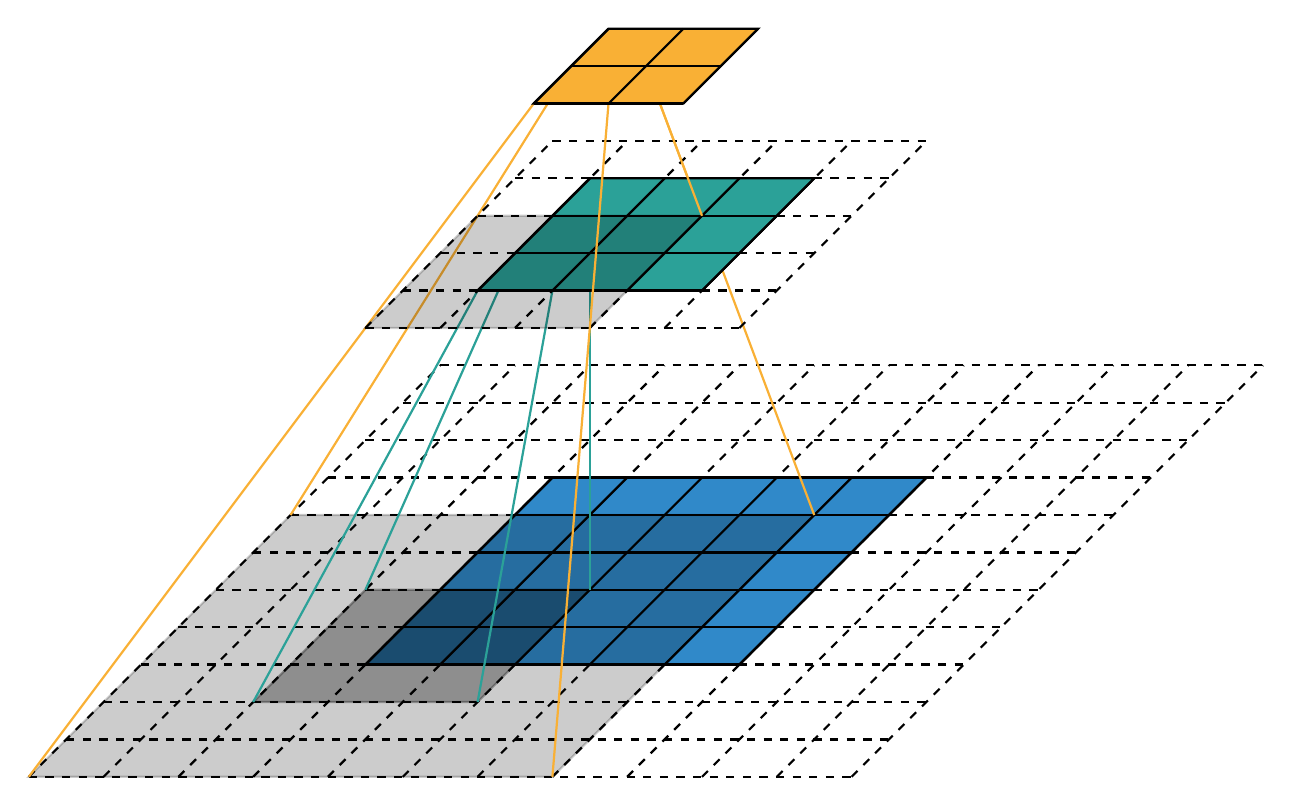
\begin{tikzpicture}[thick, scale=.95]
	\definecolor{blue}{RGB}{48, 137, 201};
\definecolor{cyan}{RGB}{43, 161, 152};
\definecolor{orange}{RGB}{249, 176, 53};

% \drawtile#x#y#size#color#opacity
\def\drawtile#1#2#3#4#5{
	\filldraw[fill=#4, opacity=#5] 
		(#1, #2) -- (#1 + #3, #2) -- (#1 + 1.5 * #3, #2 + #3 / 2) -- (#1 + #3 / 2, #2 + #3 / 2) -- cycle;
}

% \drawgrid#x#y#size#style
\def\drawgrid#1#2#3#4{
	\foreach \i in {0, ..., #3}{
		\draw[#4] (#1 + \i, #2) -- (#1 + \i + #3 / 2, #2 + #3 / 2); % vertical line
		\draw[#4] (#1 + \i / 2, #2 + \i / 2) -- (#1 + \i / 2 + #3, #2 + \i / 2); % horizontal line
	}
}

% \drawline#x1#y1#x2#y2#color
\def\drawline#1#2#3#4#5{
	\draw[#5] (#1, #2) -- (#3, #4);
}
	
	% layer 1
	\drawgrid{0}{0}{11}{dashed}
	\drawtile{4.5}{1.5}{5}{blue}{1.0}
	\drawgrid{4.5}{1.5}{5}{}
	\drawtile{0}{0}{7}{black}{0.2}
	\drawtile{3}{1}{3}{black}{0.3}
	
	% background connection
	\drawline{3}{1}{6}{6.5}{cyan}
	\drawline{6}{1}{7}{6.5}{cyan}
	\drawline{4.5}{2.5}{6.5}{7}{cyan}
	\drawline{7.5}{2.5}{7.5}{7}{cyan}
	\drawline{0}{0}{6.75}{9}{orange}
	\drawline{3.5}{3.5}{7.25}{9.5}{orange}
	\drawline{10.5}{3.5}{8.25}{9.5}{orange}
	
	% layer 2
	\drawgrid{4.5}{6}{5}{dashed}
	\drawtile{6}{6.5}{3}{cyan}{1.0}
	\drawgrid{6}{6.5}{3}{}
	\drawtile{4.5}{6}{3}{black}{0.2}
	
	% foreground connnection
	\drawline{9}{7.5}{8.25}{9.5}{orange}
	\drawline{7}{0}{7.75}{9}{orange}
	
	% layer 3
	\drawtile{6.75}{9}{2}{orange}{1.0}
	\drawgrid{6.75}{9}{2}{}
\end{tikzpicture}
% 		\caption[Receptive field của phép toán Convolution có kích thước filter $3\times 3$, stride 2 và padding ``same''.]{Receptive field của phép toán convolution\index{Convolution} có kích thước filter\index{Filter} $3\times 3$, stride\index{Stride} 2  và padding\index{Padding} ``same''\sourcefig{\cite{le2017receptive}}.}
% 		\label{fig:receptive_field}
% 	\end{figure}

% \subsection{Lớp Batchnorm}
% \label{subsec:lop_batchnorm}
% 	Thông thường chúng ta chuẩn hoá dữ liệu đầu vào bằng cách điều chỉnh và co giãn miền giá trị của chúng để việc học không bị thiên vị về một thuộc tính bất kỳ nào của dữ liệu. Ví dụ, nếu dữ liệu của chúng ta có một thuộc tính với miền giá trị trong khoảng từ 0 đến 1\linebreak và một thuộc tính khác có miền giá trị trong khoảng từ 0 đến 1000 thì chúng ta nên thực hiện bước chuẩn hoá dữ liệu để việc huấn luyện đạt kết quả tốt hơn. Tuy nhiên việc chuẩn hoá này chỉ mới được áp dụng trên dữ liệu đầu vào. Ioffe và Szegedy \cite{ioffe2015batch} đã đề xuất việc chuẩn hoá dữ liệu nên được thực hiện trên cả những lớp ẩn của kiến trúc mạng.
	
% 	Dữ liệu sẽ được chuẩn hoá nhờ lớp batchnorm\index{Batchnorm} trước khi đi qua một lớp mạng, giúp việc học trên từng lớp mạng có tính độc lập cao hơn, ít bị phụ thuộc bởi giá trị đầu ra của lớp mạng phía trước như trước đây. Đồng thời, việc sử dụng batchnorm cho phép chúng ta sử dụng giá trị learning rate\index{Learning rate} (tốc độ học) lớn hơn vì lớp batchnorm đảm bảo dữ liệu đầu vào của một lớp mạng không quá cao hoặc quá thấp.
	
% 	Lớp batchnorm thực hiện chuẩn hoá dữ liệu đầu ra của một lớp mạng bằng cách lấy giá trị đầu ra trừ đi giá trị trung bình (mean\index{Mean}) rồi chia cho độ lệch chuẩn (standard deviation) của chính nó. Chi tiết về giải thuật batchnorm được mô tả trong \autoref{fig:batchnorm}.
% 	\begin{figure}[h!]
% 		\centering
% 		\fbox{%
% 			\parbox{.6\textwidth}{%
% 				\vspace{-4mm}
% 				\begin{tabbing}
% 					\hspace{2cm}\=\kill
% 					\textbf{Input:} \>Values of $x$ over a mini-batch: $\mathcal{B}=\{x_{1...m}\}$;\\
% 					\>Parameters to be learned: $\gamma, \beta$\\
% 					\textbf{Output:} \>$\{y_i=\text{BN}_{\gamma,\beta}(x_i)\}$
% 				\end{tabbing}
% 				\begin{tabbing}
% 					\hspace{5mm}\=\hspace{6mm}\=\hspace{5mm}\=\hspace{4cm}\=\kill
% 					\>$\mu_\mathcal{B}$\>$\leftarrow$\>$\dfrac{1}{m}\sum\limits_{i=1}^{m}x_i$\>//mini-batch mean\\[3mm]
% 					\>$\sigma_\mathcal{B}^2$\>$\leftarrow$\> $\dfrac{1}{m}\sum\limits_{i=1}^{m}(x_i-\mu_\mathcal{B})^2$\>//mini-batch variance\\[3mm]
% 					\>$\hat{x}_i$\>$\leftarrow$\>$\dfrac{x_i-\mu_\mathcal{B}}{\sqrt{\sigma_\mathcal{B}^2+\epsilon}}$\>// normalize\\[3mm]
% 					\>$y_i$\>$\leftarrow$\>$\gamma\hat{x}_i+\beta\equiv\text{BN}_{\gamma, \beta}(x_i)$\>// scale and shift
% 				\end{tabbing}
% 			}%
% 		}
% 		\caption[Giải thuật Batchnorm áp dụng lên dữ liệu đầu vào của một mini-batch.]{Giải thuật Batchnorm áp dụng lên dữ liệu đầu vào của một mini-batch trong quá trình huấn luyện \sourcefig{\cite{ioffe2015batch}}.}
% 		\label{fig:batchnorm}
% 	\end{figure}

% \newpage
% \subsection{Lớp Sigmoid}
% \label{subsec:lop_sigmoid}
% 	Trong toán học, hàm sigmoid\index{Sigmoid} với phương trình toán học như sau
% 	\begin{equation}
% 	\sigma(x)=\dfrac{1}{1+e^{-x}}
% 	\label{eqn:sigmoid}
% 	\end{equation}
% 	là một hàm số biến một giá trị thực bất kỳ thành một giá trị thực trong phạm vi $(0, 1)$. Một số dương càng lớn sẽ cho ra giá trị gần với 1 và một số âm càng nhỏ sẽ cho ra giá trị gần với 0. Hàm sigmoid có thể được sử dụng sau một lớp convolution\index{Convolution} hoặc là lớp cuối cùng của kiến trúc mạng nhằm mục đích phân loại. Đồ thị biểu diễn hàm sigmoid được mô tả như \autoref{fig:sigmoid}.
% 	\begin{figure}[h!]
% 		\centering
% 		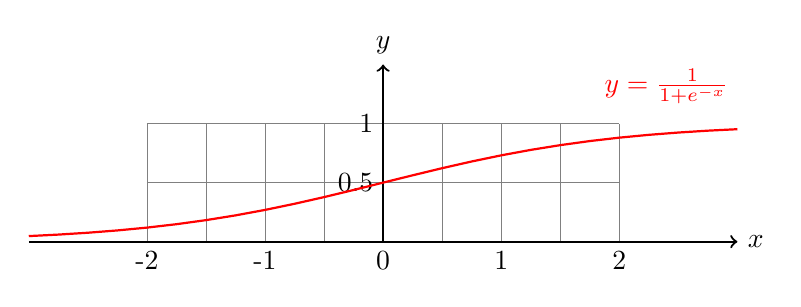
\begin{tikzpicture}[domain=-3:3, scale=1.5]
	% grid
	\draw[step=.5, very thin, color=gray] (-2, 0) grid (2, 1);
	
	% axes
	\draw[->,thick] (-3, 0) -- (3, 0) node[right] {$x$};
	\draw[->,thick] (0, 0) -- (0, 1.5) node[above] {$y$};
	\foreach \x in {-2, ..., 2}
		\node[anchor=north] at (\x, 0) {\x};
	\foreach \y in {0.5, 1}
		\node[anchor=east] at (0, \y) {\y};
		
	% sigmoid function
	\draw[thick, color=red] plot (\x, {1 / (1 + e^-\x)}) 
		node[anchor=north,  xshift=-9mm, yshift=9mm] {$y=\frac{1}{1+e^{-x}}$};
\end{tikzpicture}
% 		\caption{Đồ thị biểu diễn hàm sigmoid.}
% 		\label{fig:sigmoid}
% 	\end{figure}
% 	\vspace{-6mm}

% \subsection{Lớp ReLU}
% \label{subsec:lop_relu}
% 	ReLU (Rectified Linear Unit)\index{ReLU} do Mair và Hinton \cite{nair2010rectified} đề xuất với công thức toán học\linebreak như sau 
% 	\begin{equation}
% 		ReLU(x)=max(0, x),
% 		\label{eqn:relu}
% 	\end{equation}
% 	nghĩa là hàm ReLU đặt một ngưỡng tại 0 chỉ cho những giá trị dương đi qua. So với hàm Sigmoid\index{Sigmoid}, hàm ReLU giúp tăng tốc độ hội tụ khi huấn luyện bằng SGD (Stochastic Gradient Descent)\index{SGD}\nomenclature{SGD}{Stochastic Gradient Descent}. Một ưu điểm nữa của hàm ReLU là trong quá trình lập trình, hàm ReLU có thể hiện thực dễ dàng bằng cách áp một mặt nạ với ngưỡng bằng 0 cho cả quá trình lan truyền xuôi và lan truyền ngược. Tuy nhiên, chính việc áp mặt nạ làm cho gradient bằng $0$ tại một số điểm trong mạng dẫn đến gradient\index{Gradient} từ điểm đó về trước trong quá trình lan truyền ngược bằng $0$ và mạng không học được. Đồ thị biểu diễn hàm ReLU như \autoref{fig:relu}.
% 	\begin{figure}[h!]
% 		\centering
% 		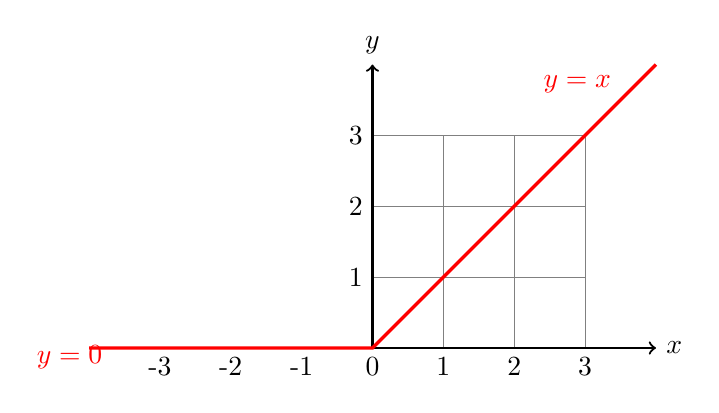
\begin{tikzpicture}[domain=-4:4, scale=.9]
	% grid
	\draw[very thin, color=gray] (0, 0) grid (3, 3);
	
	% axes
	\draw[->,thick] (-4, 0) -- (4, 0) node[right] {$x$};
	\draw[->,thick] (0, 0) -- (0, 4) node[above] {$y$};
	\foreach \x in {-3, ..., 3}
		\node[anchor=north] at (\x, 0) {\x};
	\foreach \y in {1, ..., 3}
		\node[anchor=east] at (0, \y) {\y};
		
	% relu function
	\draw[very thick, color=red] plot (\x, { max(0, \x) }) 
		node[anchor=north,  xshift=-1cm] {$y=x$}
		node[anchor=south west, xshift=-8cm, yshift=-4cm] {$y=0$};
\end{tikzpicture}
% 		\caption{Đồ thị biểu diễn hàm ReLU.}
% 		\label{fig:relu}
% 	\end{figure}

% \subsection{Lớp Softmax}
% \label{subsec:lop_softmax}
% 	Trong toán học, hàm softmax\index{Softmax} (hay hàm trung bình mũ) là một hàm số biến không gian $K$ chiều với giá trị thực bất kỳ đến không gian $K$ chiều mang giá trị trong phạm vi $(0, 1)$. Phương trình toán học của hàm softmax được biểu diễn như sau
% 	\begin{equation}
% 	a_i=\dfrac{e^{z_i}}{\sum_{j=1}^{K}e^{z_j}},
% 	\label{eqn:softmax}
% 	\end{equation}
% 	trong đó, $z_i$ là giá trị đầu vào, $K$ là số khả năng khác nhau có thể xảy ra và $a_i$ là giá trị đầu ra của hàm softmax. Hàm softmax là một hàm đồng biến đảm bảo nếu giá trị $z_i$ càng lớn thì xác suất rơi vào khả năng thứ $i$ trong $K$ khả năng càng cao. Đồng thời, hàm này đảm bảo các giá trị đầu ra $a_i$ dương và tổng của chúng bằng $1$. \autoref{fig:softmax} mô tả một số giá trị đầu vào và đầu ra tương ứng của hàm softmax.
% 	\begin{figure}[h!]
% 		\centering
% 		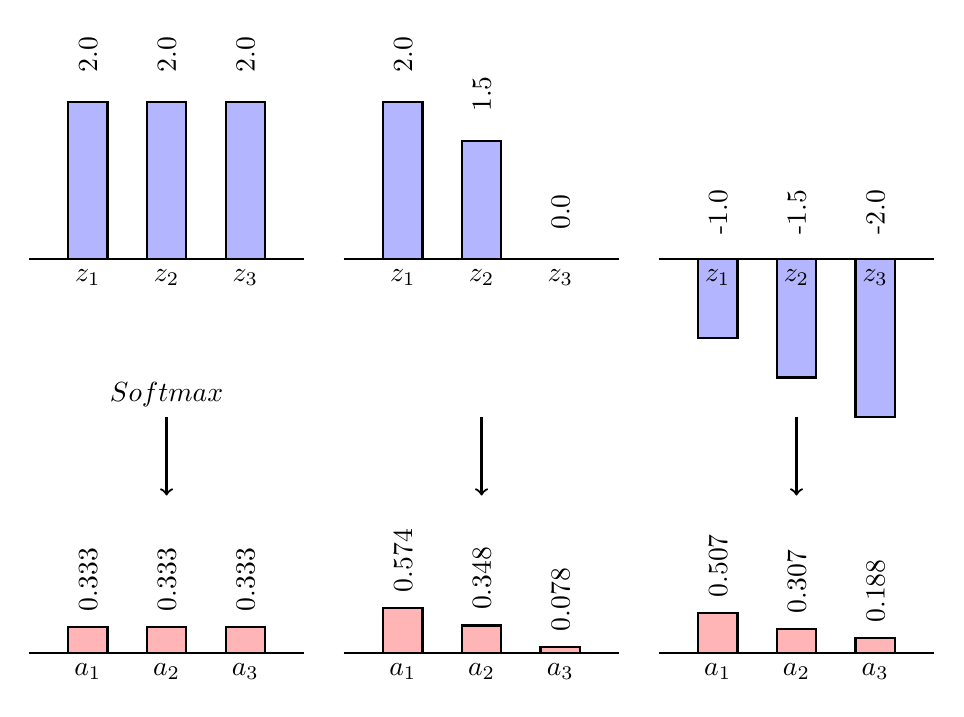
\begin{tikzpicture}[thick]
	\definecolor{incolor}{RGB}{180, 181, 255}
	\definecolor{outcolor}{RGB}{255, 181, 181}
	
	% \drawcol#x#y#value#label#color
	\def\drawcol#1#2#3#4#5{
		\filldraw[fill=#5] (#1, {min(#2, #2 + #3)}) rectangle (#1 + .5, {max(#2, #2 + #3)}) 
			node[above, rotate=90, xshift=6mm] {#3};
		\node[anchor=north] at (#1 + .25, #2) {#4};
	}

	% \drawbar#x#y#value1#value2#value3#label#color
	\def\drawbar#1#2#3#4#5#6#7{
		\draw (#1, #2) -- (#1 + 3.5, #2);
		\drawcol{#1 + 0.5}{#2}{#3}{$#6_1$}{#7}
		\drawcol{#1 + 1.5}{#2}{#4}{$#6_2$}{#7}
		\drawcol{#1 + 2.5}{#2}{#5}{$#6_3$}{#7}
	}
	
	% input
	\drawbar{0}{5} { 2.0}{ 2.0}{ 2.0} {z} {incolor}
	\drawbar{4}{5} { 2.0}{ 1.5}{ 0.0} {z} {incolor}
	\drawbar{8}{5} {-1.0}{-1.5}{-2.0} {z} {incolor}
	
	% down arrow
	\draw[->] (1.75, 3) node[above] {$Softmax$} -- (1.75, 2) ;
	\draw[->] (5.75, 3) -- (5.75, 2);
	\draw[->] (9.75, 3) -- (9.75, 2);
	
	% output
	\drawbar{0}{0} {0.333}{0.333}{0.333} {a} {outcolor}
	\drawbar{4}{0} {0.574}{0.348}{0.078} {a} {outcolor}
	\drawbar{8}{0} {0.507}{0.307}{0.188} {a} {outcolor}
\end{tikzpicture}
% 		\caption[Một số ví dụ về đầu vào và đầu ra của hàm Softmax.]{Một số ví dụ về đầu vào và đầu ra của hàm Softmax \sourcefig{\cite{machinelearningcoban}}.}
		
% 		\label{fig:softmax}
% 	\end{figure}
	
% 	Trong lý thuyết xác suất, giá trị xuất ra của hàm softmax có thể được sử dụng để đại diện cho một loại phân phối -- đó là phân phối xác suất trên $K$ khả năng khác nhau có thể xảy ra.
	
% 	Hàm softmax\index{Softmax} được sử dụng trong nhiều phương pháp phân loại đa lớp như hồi quy logistic đa biến, biệt thức tuyến tính phân tích nhiều lớp và mạng nơ-ron. Đặc biệt, trong mạng nơ-ron, lớp softmax được sử dụng làm lớp cuối cùng của kiến trúc mạng để xác định độ chắc chắc trong kết quả dự đoán.
	
\newpage
\section{Machine Learning Model} 
\label{sec:machine_model}
	
\subsection{Logistic Regression}
\label{subsec:logistic_regression}
\subsubsection{Logistic Regression Model}
Predictive output of Linear Regression:
\begin{align}
	f(x) = w^T x
\end{align}

\subsubsection{Sigmoid Function}
Sigmoid function:
\begin{align}
    f(s) = \frac{1}{1 + e^{-s}} \triangleq \sigma(s)
\end{align}

\subsubsection{Optimize loss function}
The Stochastic Gradient Descent (SGD) algorithm will be used here.

\begin{align}
    \frac{\partial z}{z(1-z)} = \partial s \newline
	\Leftrightarrow (\frac{1}{z} + \frac{1}{1 - z})\partial z = \partial s \newline
\end{align}

\subsection{Phép toán Skeleton}
\label{subsec:phep_toan_skeleton}
	Phép toán trích xuất khung xương đối tượng skeleton\index{Skeleton} là một trong các phép toán biến đổi hình thái được giới thiệu bởi Fisher và cộng sự \cite{hipr2thining}. Phép toán này được sử dụng để rút trích thành phần chính đại diện cho hình dạng của đối tượng trong ảnh nhị phân. Được ứng dụng trong nhận dạng mẫu (nhận dạng kí tự), nén ảnh, phát hiện lỗi trên sản phẩm công nghiệp (đứt đoạn).
	
	Gọi $\{nB\}, n= 0, 1, ...$ là một họ các hình khối với $B$ là một thành phần cấu trúc, ta có
	\begin{equation}
		nB = \underbrace{B\oplus \cdots \oplus B}_{n\ \text{lần}}.
		\label{eqn:skeleton_nb}
	\end{equation}
	Khi $n=0$, $nB=\{o\}$ với $o$ biểu diễn cho thành phần cấu trúc ban đầu. Phép toán skeleton lên ảnh nhị phân $A$ được định nghĩa như sau
	\begin{equation}
		S(A) = \bigcup_{n = 0}^N (A \ominus nB) - ((A \ominus nB) \ominus B)\oplus B,
		\label{eqn:skeleton}
	\end{equation}
	trong đó, $N$ là số lần lặp lớn nhất trước khi $A$ trở thành tập rỗng. $N$ được xác định theo công thức
	\begin{equation}
		N = \text{max}\{k|(A\ominus kB)\neq\varnothing\}.
	\label{eqn:skeleton_n}
	\end{equation}
	
	\autoref{fig:skeleton2d_apply} là một ví dụ áp dụng phép toán skeleton để rút trích khung xương đối tượng trong ảnh nhị phân.
	\begin{figure}[h!]
		\hfill
		\begin{subfigure}[b]{0.475\textwidth}
			\centering
			\begin{tikzpicture}[thick, scale=.45]
	\def\colors{{
		"000 000 000", % black
		"255 255 255"  % white
	}}

	% \drawsquare#x#y#label#textcolor#fillcolor
	\def\drawsquare#1#2#3#4#5{
		\filldraw[fill=#5] (#1, #2) rectangle (#1 + 1, #2 + 1) node[pos=.5] {\textcolor{#4}{\scriptsize #3}};
	}
	
	% values
	\def\values{{
		0, 0, 0, 0, 0, 0, 0, 0, 0, 0, 0, 0, 0, 0, 0, 0,
		0, 0, 0, 0, 0, 0, 0, 0, 0, 0, 0, 0, 0, 0, 0, 0,
		0, 1, 1, 0, 0, 0, 0, 0, 0, 0, 0, 0, 0, 0, 0, 0,
		0, 0, 0, 1, 0, 0, 0, 1, 0, 0, 0, 0, 0, 0, 0, 0,
		0, 0, 1, 1, 1, 1, 1, 1, 1, 1, 0, 0, 0, 0, 0, 0,
		0, 0, 1, 1, 1, 1, 1, 1, 1, 1, 1, 1, 0, 0, 0, 0,
		0, 0, 1, 1, 1, 1, 1, 1, 1, 1, 1, 1, 1, 0, 0, 0,
		0, 0, 1, 1, 1, 1, 1, 1, 1, 1, 1, 1, 1, 1, 0, 0,
		0, 0, 1, 1, 1, 0, 0, 0, 0, 1, 1, 1, 1, 1, 0, 0,
		0, 0, 1, 1, 0, 0, 0, 0, 0, 0, 1, 1, 1, 1, 0, 0,
		0, 0, 1, 1, 0, 0, 0, 0, 0, 0, 0, 1, 1, 1, 0, 0,
		0, 0, 1, 0, 0, 0, 0, 0, 0, 0, 0, 0, 1, 1, 0, 0,
		0, 0, 1, 0, 0, 0, 0, 0, 0, 0, 0, 0, 1, 1, 0, 0,
		0, 0, 1, 0, 0, 0, 0, 0, 0, 0, 0, 0, 0, 1, 0, 0,
		0, 0, 0, 1, 1, 1, 0, 0, 0, 0, 0, 0, 0, 0, 0, 0,
		0, 0, 0, 0, 0, 0, 0, 0, 0, 0, 0, 0, 0, 0, 0, 0,
	}}
	
	% pixel
	\foreach \y in {0, ..., 15} {
		\foreach \x in {0, ..., 15} {
			\def\value{\values[16 * \y + \x]}
			\pgfmathparse{\colors[\value]};
			\definecolor{fillcolor}{RGB}{\pgfmathresult};
			\pgfmathparse{\colors[1 - \value]};
			\definecolor{textcolor}{RGB}{\pgfmathresult};
			\drawsquare{\x}{15 - \y}{\pgfmathparse{\value}\pgfmathresult}{textcolor}{fillcolor}
		}
	}
\end{tikzpicture}
			\caption{}
			\label{fig:skeleton2d_apply_before}
		\end{subfigure}
		\begin{subfigure}[b]{0.475\textwidth}
			\centering
			\begin{tikzpicture}[thick, scale=.45]
	\def\colors{{
		"000 000 000", % black
		"255 255 255"  % white
	}}

	% \drawsquare#x#y#label#textcolor#fillcolor
	\def\drawsquare#1#2#3#4#5{
		\filldraw[fill=#5] (#1, #2) rectangle (#1 + 1, #2 + 1) node[pos=.5] {\textcolor{#4}{\scriptsize #3}};
	}
	
	% values
	\def\values{{
		0, 0, 0, 0, 0, 0, 0, 0, 0, 0, 0, 0, 0, 0, 0, 0,
		0, 0, 0, 0, 0, 0, 0, 0, 0, 0, 0, 0, 0, 0, 0, 0,
		0, 1, 1, 0, 0, 0, 0, 0, 0, 0, 0, 0, 0, 0, 0, 0,
		0, 0, 0, 1, 0, 0, 0, 0, 0, 0, 0, 0, 0, 0, 0, 0,
		0, 0, 0, 1, 0, 0, 0, 0, 0, 0, 0, 0, 0, 0, 0, 0,
		0, 0, 0, 1, 0, 0, 0, 0, 0, 0, 0, 0, 0, 0, 0, 0,
		0, 0, 0, 1, 0, 0, 0, 1, 1, 0, 0, 0, 0, 0, 0, 0,
		0, 0, 0, 1, 1, 1, 1, 0, 0, 1, 0, 0, 0, 0, 0, 0,
		0, 0, 0, 1, 0, 0, 0, 0, 0, 0, 1, 0, 0, 0, 0, 0,
		0, 0, 0, 1, 0, 0, 0, 0, 0, 0, 0, 1, 0, 0, 0, 0,
		0, 0, 0, 1, 0, 0, 0, 0, 0, 0, 0, 0, 1, 0, 0, 0,
		0, 0, 1, 0, 0, 0, 0, 0, 0, 0, 0, 0, 1, 0, 0, 0,
		0, 0, 1, 0, 0, 0, 0, 0, 0, 0, 0, 0, 1, 1, 0, 0,
		0, 0, 1, 0, 0, 0, 0, 0, 0, 0, 0, 0, 0, 1, 0, 0,
		0, 0, 0, 1, 1, 1, 0, 0, 0, 0, 0, 0, 0, 0, 0, 0,
		0, 0, 0, 0, 0, 0, 0, 0, 0, 0, 0, 0, 0, 0, 0, 0,
	}}
	
	% pixel
	\foreach \y in {0, ..., 15} {
		\foreach \x in {0, ..., 15} {
			\def\value{\values[16 * \y + \x]}
			\pgfmathparse{\colors[\value]};
			\definecolor{fillcolor}{RGB}{\pgfmathresult};
			\pgfmathparse{\colors[1 - \value]};
			\definecolor{textcolor}{RGB}{\pgfmathresult};
			\drawsquare{\x}{15 - \y}{\pgfmathparse{\value}\pgfmathresult}{textcolor}{fillcolor}
		}
	}
\end{tikzpicture}
			\caption{}
			\label{fig:skeleton2d_apply_after}
		\end{subfigure}
		\hfill\null
		\caption[Áp dụng phép toán Skeleton để rút trích khung xương đối tượng trong không gian 2D.]{Áp dụng phép toán Skeleton để rút trích khung xương đối tượng trong không gian 2D. \subref{fig:skeleton2d_apply_before} ảnh nhị phân ban đầu. \subref{fig:skeleton2d_apply_after} ảnh nhị phân sau khi trích xuất khung xương đối tượng. \sourcefig{\cite{hipr2thining}}.}
		\label{fig:skeleton2d_apply}
	\end{figure}
	
	Trong luận văn này chúng tôi sử dụng kỹ thuật rút trích khung xương đối tượng trong không gian 3D được đề xuất bởi Lee và cộng sự \cite{lee1994building} để tìm đường chính giữa của mạch máu trong \autoref{sec:tim_duong_chinh_giua_va_diem_phan_nhanh}. \autoref{fig:skeleton3d_apply} minh hoạ việc áp dụng phép toán skeleton làm mảnh đối tượng trong không gian 3D.
	\begin{figure}[h!]
		\centering
		\begin{subfigure}[b]{0.49\textwidth}
			\centering
			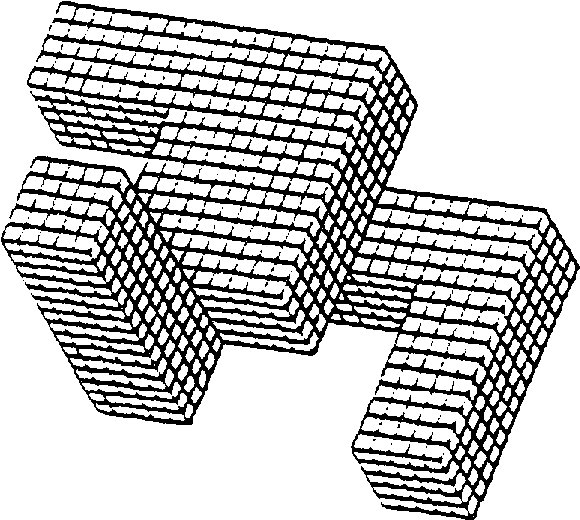
\includegraphics[width=.8\textwidth]{figures/morphology_skeleton3d_before}
			\caption{}
			\label{fig:skeleton3d_apply_before}
		\end{subfigure}
		\hfill
		\begin{subfigure}[b]{0.49\textwidth}
			\centering
			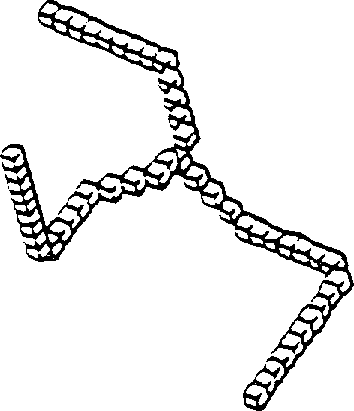
\includegraphics[width=.6\textwidth]{figures/morphology_skeleton3d_after}
			\caption{}
			\label{fig:skeleton3d_apply_after}
		\end{subfigure}%
		\caption[Áp dụng phép toán Skeleton để rút trích khung xương đối tượng trong không gian 3D.]{Áp dụng phép toán Skeleton để rút trích khung xương đối tượng trong không gian 3D. \subref{fig:skeleton3d_apply_before} đối tượng ban đầu. \subref{fig:skeleton3d_apply_after} khung xương được tạo ra từ phép toán skeleton. \sourcefig{\cite{lee1994building}}.}
		\label{fig:skeleton3d_apply}
	\end{figure}

\section{Thư viện và công cụ} 
\label{sec:thu_vien_va_cong_cu}
	Trong mục này, chúng tôi giới thiệu các thư viện và công cụ mà chúng tôi đã sử dụng trong quá trình thực hiện Luận văn này, bao gồm nền tảng PyTorch, thư viện VTK và ứng dụng Slicer.

\subsection{Nền tảng PyTorch}
\label{subsec:nen_tang_pytorch}
	\index{PyTorch}PyTorch\footnote{\url{https://pytorch.org}}là một nền tảng mã nguồn mở được phát triển và duy trì bởi nhóm nghiên cứu về trí thông minh nhân tạo của Facebook. PyTorch có khả năng tự động ghi lại các toán tử đã xử lý vào một đồ thị tính toán trong bước forward\index{Forward} (lan truyền xuôi) và sau đó tái thực thi các toán tử này để tính toán gradient\index{Gradient} một cách nhanh chóng ở bước backward\index{Backward} (lan truyền ngược). Kỹ thuật này giúp PyTorch trở nên hiệu quả trong việc xây dựng một mạng nơ-ron vì nó giúp tiết kiệm thời gian nhờ vào việc tính toán đạo hàm các tham số trước khi thực hiện bước forward. Với phiên bản mới nhất của PyTorch (phiên bản 1.0.1, xem \cite{Soumith2019}), các nhà phát triển có thể chuyển từ giai đoạn nghiên cứu sang giai đoạn triển khai sản phẩm một cách dễ dàng, biến PyTorch trở thành một nền tảng học sâu vô cùng mạch mẽ. PyTorch được viết bằng ngôn ngữ C++, CUDA\nomenclature{CUDA}{Compute Unified Device Architecture} và Python và được tối ưu hoá hoàn toàn cho các tác vụ học sâu trên cả CPU\nomenclature{CPU}{Central Processing Unit} và GPU như xử lý hình ảnh, huấn luyện các mạng học sâu với khả năng huấn luyện song song trên nhiều GPU, v.v.
	
	Với các tính năng phong phú và sự năng động của cộng đồng hỗ trợ và phát triển, chúng tôi chọn PyTorch làm nền tảng xây dựng và phát triển hệ thống trong luận văn này.
	
\newpage
\subsection{Thư viện VTK}
\label{subsec:thu_vien_vtk}
	\nomenclature{VTK}{The Visualization Toolkit}\index{VTK}VTK (The Visualization Toolkit)\footnote{\url{https://pypi.org/project/vtk/}}là một thư viện mã nguồn mở cung cấp cho các nhà phát triển một bộ công cụ đa dạng phục vụ cho đồ hoạ máy tính trong không gian ba chiều, xử lý hình ảnh và trực quan hoá. Thư viện này được hiện thực từ nhiều ngôn ngữ khác nhau như C++, Java và Python. Nó hỗ trợ nhiều giải thuật trực quan hoá bao gồm phương pháp vô hướng, phương pháp vec-tơ, phương pháp kết cấu và thể tích. Đặc biệt, thư viện này còn hỗ trợ các kỹ thuật mô hình hoá nâng cao như mô hình ẩn, thu giảm đa giác, làm mịn bề mặt, tạo đường viền và tam giác phân Delaunay.
	
	Trong luận văn này, chúng tôi sử dụng thư viện VTK trên ngôn ngữ Python nhằm trích xuất và làm mịn lưới bề mặt hệ thống mạch máu cũng như đường chính giữa mạch máu và các điểm phân nhánh từ kết quả dự đoán, phục vụ quá trình trực quan hoá sẽ được đề cập tới trong \autoref{sec:truc_quan_hoa_ket_qua_thi_nghiem}.

\subsection{Phần mềm Slicer}
\label{subsec:pham_mem_Slicer}
	\index{Slicer}Slicer\footnote{\url{https://www.slicer.org/}}là ứng dụng mã nguồn mở phục vụ cho tin học về hình ảnh y tế, xử lý hình ảnh y khoa và trực quan hoá trong không gian ba chiều. Được xây dựng trong hơn hai thập kỷ qua với sự hỗ trợ của các viện y tế quốc gia (National Institutes of Health) và cộng đồng các nhà phát triển trên toàn thế giới, trong đó phải kể đến sự đóng góp của cộng đồng quốc tế các nhà khoa học, bao gồm cả kỹ thuật và y sinh. Slicer mang đến các công cụ xử lý đa nền tảng miễn phí, mạnh mẽ cho các bác sĩ, các nhà nghiên cứu và cộng đồng.
	
	Trong luận văn này, chúng tôi sử dụng ứng dụng Slicer để trực quan hoá kết quả thu được từ hệ thống, nhằm đưa ra những nhận xét mang tính định tính chất lượng, giúp kết quả đánh giá được toàn diện hơn. Chúng tôi sẽ đề cập rõ hơn trong \autoref{sec:truc_quan_hoa_ket_qua_thi_nghiem}.